\section{Introduction}
The Internet of Things (IoT) is one of the research and industrial fields that faced the most rapid growth in the recent years, mostly thanks to the proliferation of new technologies associated with the ease of installation and use.
This development has created a wide variety of standards and solutions at each layer of the network and application stack, leading to an heterogeneous environment both in terms of communication technologies and data storage.
This results in disconnected network islands, in which it is easy to build networks with homogeneous devices, however it is hard to integrate data provided by other sources.
Since the beginning of its diffusion, its potential has been explored in various fields of application and its major usefulness has been claimed to be in service composition and interoperability \cite{atzori2010internet}. The requirements when designing collaborative IoT-related automation systems are varying due to the heterogeneity of the platforms and the hardware components as well as the network interfaces.
This resulted in a sparse set of technologies and terminologies used in several scenarios determining a lack of interoperability among systems.
The common approach to the problem of unifying entities within an ecosystem is typically architectural and leads to a difficult reuse of the components among different solutions \cite{krco2014designing}.
To face these issues the European Commission supported initiatives like IoT-A \cite{iot-a}, which aimed to release an architectural reference model, and FI-WARE \cite{fiware}, which also helped architects in establishing a unified vision and nomenclature and now had become an implementation-driven open community.
FI-WARE also provided a sandbox, in which partners could upload their open data, although it is not of broad use nowadays.
Such solutions, unfortunately, did not solve the problem introduced by architectures, in fact different approaches still tend to create separate ecosystems which are hard to unify.

At the same time, makers worldwide build their own IoT in-home networks, which provide a low cost and customized environment that suit their needs.
Platforms like Arduino \cite{arduino} and Raspberry Pi \cite{raspberry} have demonstrated their ease of use and they fit most of the needs of citizens willing to build their own network.
However, certain types of sensor can be too expensive, or cannot be deployed due to restrictions or physical space limitations.
For this reason, collaborative IoT is seen as a useful solution that facilitates the access to critical data.

In this paper we aim to show the usefulness and the potential of open data exploitation for global cooperative IoT automation scenarios.
As a preliminary approach, we focused our analyses on data coming from two of the main open data platforms for sensors, ThingSpeak \cite{thingspeak} and SparkFun \cite{sparkfun}, which provide open data uploaded by privates and coming from different types of sensors, along with temporal and, possibly, positional information.
Such parameters can tell us much about the general trend in the usage of these platforms throughout a time window of few years.
Each data stream in both platforms comes with a creation date, which we reported, after a data extraction, in the diagram in Figure~\ref{creationtrend}.

\begin{figure}[btp]
\centering
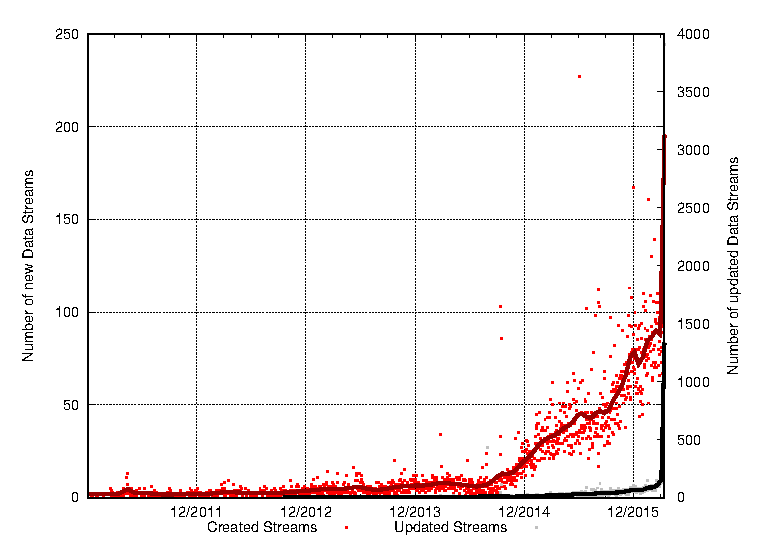
\includegraphics[width=0.48\textwidth]{img/bars.eps} 
\caption{Trend in creation and update of ThingSpeak channels.}
\label{creationtrend}
\end{figure}

Starting from such analysis it results a substantial growth in created channels starting from the end of 2014. 
A possible intuition behind this phenomenon is the parallel innovation in simple hardware modules, for instance August 2014 corresponds to the launch of the first version of ESP8266 \cite{esp8266} on the market and in October 2014 was possible to flash its firmware though an SDK \cite{espressif}.
In the same figure we also reported the time of the last update for all the found streams.
The oldest updates we found fall back to 2012, therefore we do not have any information on streams that were updated for the last time before that date.
The steepness of the curve in the last days reveals that a significant amount of the data streams are still in use and updated daily or even hourly, and can therefore provide fresh information.
Such analyses shed some light on how rapidly the world of open data is growing and people are gaining interest in using a platform that takes away the burden of creating a local ecosystem.
Thus, our work creates the basis for a solid global ecosystem with a strong impact on cooperative services, integrating data coming from custom made solutions with reliable data sources.
Indeed, we use the terms ``reliable'' and ``unreliable'' to identify, respectively, data sources labeled as official, such as data provided by the government, and data sources generated by users, which do not need to be confirmed by a trustworthy entity. 

The rest of this paper is structured as follows: In Section \ref{sec:rel} we present similar works from literature; Section \ref{sec:open} describes the data stream examples we considered for this analysis, and Section \ref{sec:unification} is devoted to the description on how it is possible to integrate heterogeneous data and the challenges on the topic; Section \ref{sec:casestudy} describes our proposed architecture, and Section \ref{sec:conclusions} concludes this paper.